\documentclass{article}
\usepackage[english]{babel}
\usepackage{blindtext}
\usepackage[margin=2.5cm]{geometry}
\usepackage{graphicx}
\graphicspath{ {./images/} }

\usepackage{tabularx}

\title{Report Assignment 1}
\author{Fabrizio Rossi, Mina Makar, Matteo Orsini}
\date{\today}

\begin{document}

\begin{titlepage}
\clearpage\maketitle
\thispagestyle{empty}
\end{titlepage}

\section*{Question 1.d}

\begin{enumerate}
\item \textbf{First $Gx$, then $Gx^T$}

In this image we can see that applying the convolution of a 1D Gaussian along the x-axis ($G_x$) and then along the y-axis ($G_x^T$) we get a 2D Gaussian filter based on the Gaussian separability property, which implies that a $n$ dimensional Gaussian convolution is equivalent to $n$ 1D Gaussian convolutions, so convolving $Gx$ over $Gx^T$ we obtain a 2D Gaussian kernel.
Based on the Gaussian separability property we can improve the performances using the following equation:
\begin{equation}
(G_x \otimes G_y) \otimes I = G_x \otimes (G_y \otimes I)
\end{equation}
where $G_x$ is the Gaussian kernel along the x-axis, $G_y$ is the Gaussian kernel along the y-axis (in our case $G_x^T$) and $I$ is the source image.

Moreover, in this case we apply first the $Gx$ kernel then the $Gy$ kernel thanks to the commutative property of the convolution operation.

\item \textbf{First $Gx$, then $Dx^T$}

Applying first the 1D Gaussian along the x-axis ($Gx$) we get a single line whose intensity follows a Gaussian distribution. Then applying the transposed derivative filter ($Dx^T$) we expand the single line vertically increasing the intensity in the top half of the image and decreasing the intensity in the bottom half. Convolving the derivative of the Gaussian function we can identify edges by looking at the maxima and minima of the function.

\item \textbf{First $Dx^T$, then $Gx$}

We obtain the same result of the previous experiment because the convolution operation is commutative, so we can first apply the derivative of the Gaussian along the y-axis and than the Gaussian along the x-axis based on the following equation:

\begin{equation}
D_x^T \otimes (G_x \otimes I) = G_x \otimes (D_x^T \otimes I)
\end{equation}

\item \textbf{First $Dx$, then $Dx^T$}

Applying the derivative kernel of a Gaussian function we can first obtain the edges along the x-axis and then reapplying the same function along the y-axis we identify the edges in both directions.

\item \textbf{First $Dx$, then $Gx^T$}

We obtain the same result of the second experiment just with swapped axis, since we used the derivative along the x-axis and the Gaussian function along the y-axis.

\item \textbf{First $Gx^T$, then $Dx$}

As we said earlier, the convolution operation is commutative so we obtain the same result as the experiment before.

\end{enumerate}

\section*{Question 1.e}

Convolving the images with the Dx kernel we can identify edges along the x-axis because the derivative of the image increases the gap between low and high values, creating new maxima and minima, allowing us to detect edges by looking at them. The same effect can be obtained using Dy along the y-axis.

Instead, if we compute the gradient of the two derivatives we can roughly detect edges in the original image in all directions. We use the gradient because its direction of the gradient is perpendicular to the edges and its magnitude represents the edge strength.
But the edges are too broad and they not follow the requirement of good localization for an edge detector, so to obtain better results we should apply a thinning technique, like the non-maximum suppression in the Canny operator.

In our case, we use a Gaussian function to smooth the image because since the derivative enhances noise we need to reduce it before applying the edge detection otherwise we will see a lot of edges in a noisy region.

\begin{figure}[ht]
\centering
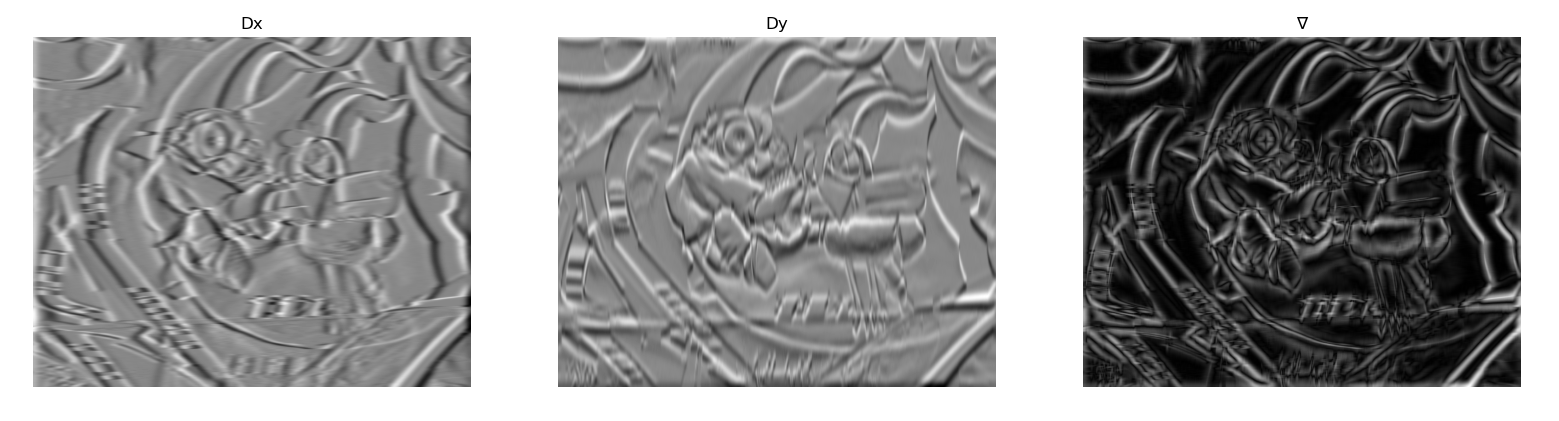
\includegraphics[width=\textwidth]{result_graf}
\caption{DxDy applied to graf.png}
\label{fig:res-graf}
\end{figure}

\begin{figure}[ht]
\centering
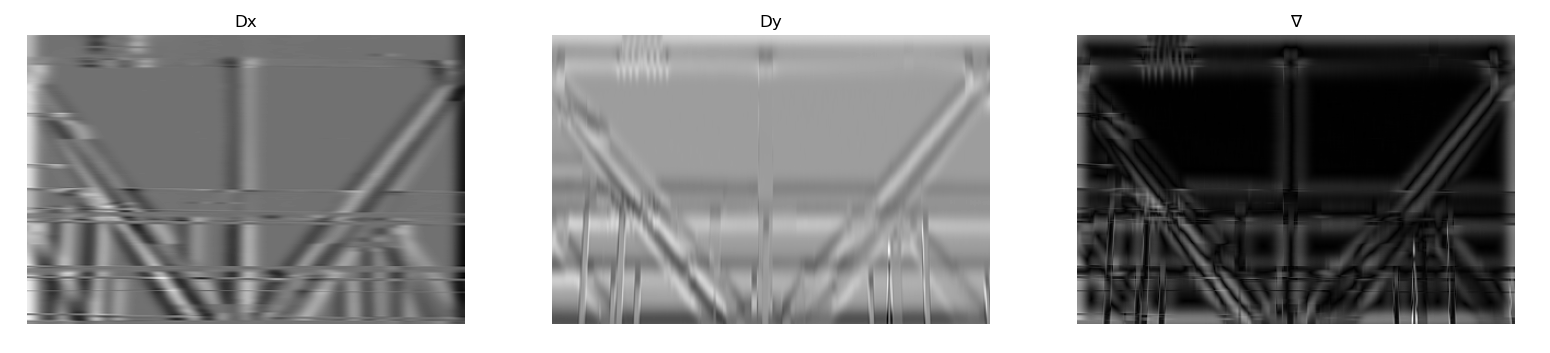
\includegraphics[width=\textwidth]{result_gantrycrane}
\caption{DxDy applied to gantrycrane.png}
\label{fig:res-gantrycrane}
\end{figure}

\section*{Question 3.c}

To conduct our experiments we evaluated the \textbf{find\_best\_match} function using the following parameters:

\begin{center}
\begin{tabularx}{.7\linewidth}{|>{\centering\arraybackslash}X|>{\centering\arraybackslash}X|>{\centering\arraybackslash}X|}
 \hline
 \multicolumn{3}{|c|}{\textbf{Distance type}}\\
 \hline
 intersect & l2 & chi2 \\
 \hline
\end{tabularx}
\end{center}

\begin{center}
\begin{tabularx}{.7\linewidth}{|>{\centering\arraybackslash}X|>{\centering\arraybackslash}X|>{\centering\arraybackslash}X|>{\centering\arraybackslash}X|}
 \hline
 \multicolumn{4}{|c|}{\textbf{Histogram type}}\\
 \hline
 greyscale & rg & rgb & dxdy \\
 \hline
\end{tabularx}
\end{center}
 
\begin{center}
\begin{tabularx}{.7\linewidth}{|>{\centering\arraybackslash}X|>{\centering\arraybackslash}X|>{\centering\arraybackslash}X|>{\centering\arraybackslash}X|>{\centering\arraybackslash}X|}
 \hline
 \multicolumn{5}{|c|}{\textbf{Number of bins}}\\
 \hline
 10 & 20 & 30 & 40 & 50 \\
 \hline
\end{tabularx}
\end{center}

And we obtained these results:

\begin{center}
\begin{tabularx}{.7\linewidth}{|>{\centering\arraybackslash}X|>{\centering\arraybackslash}X|>{\centering\arraybackslash}X|>{\centering\arraybackslash}X|>{\centering\arraybackslash}X|}
 \hline
\textbf{Distance type} & \textbf{Histogram type} & \textbf{Number of bins} & \textbf{Correct matches} & \textbf{Recognition rate}\\
 \hline
 l2 & grayvalue & 10 & 39 & 0.43\\
  \hline
l2 & grayvalue & 20 & 34 & 0.38\\
 \hline
l2 & grayvalue & 30 & 36 & 0.40\\
 \hline
l2 & grayvalue & 40 & 34 & 0.38\\
 \hline
l2 & grayvalue & 50 & 31 & 0.34\\
 \hline
l2 & rgb & 10 & 54 & 0.60\\
\hline
l2 & rgb & 20 & 42 & 0.47\\
\hline
l2 & rgb & 30 & 34 & 0.38\\
\hline
l2 & rgb & 40 & 30 & 0.33\\
\hline
l2 & rgb & 50 & 30 & 0.33\\
\hline
l2 & rg & 10 & 52 & 0.58\\
\hline
l2 & rg & 20 & 43 & 0.48\\
\hline
l2 & rg & 30 & 39 & 0.43\\
\hline
l2 & rg & 40 & 37 & 0.41\\
\hline
l2 & rg & 50 & 31 & 0.34\\
\hline
l2 & dxdy & 10 & 39 & 0.43\\
\hline
l2 & dxdy & 20 & 40 & 0.44\\
\hline
l2 & dxdy & 30 & 38 & 0.42\\
\hline
l2 & dxdy & 40 & 37 & 0.41\\
\hline
l2 & dxdy & 50 & 36 & 0.40\\
\hline
\end{tabularx}
\end{center}

\begin{center}
\begin{tabularx}{.7\linewidth}{|>{\centering\arraybackslash}X|>{\centering\arraybackslash}X|>{\centering\arraybackslash}X|>{\centering\arraybackslash}X|>{\centering\arraybackslash}X|}
 \hline
\textbf{Distance type} & \textbf{Histogram type} & \textbf{Number of bins} & \textbf{Correct matches} & \textbf{Recognition rate}\\
\hline
intersect & grayvalue & 10 & 45 & 0.50\\
\hline
intersect & grayvalue & 20 & 46 & 0.51\\
\hline
intersect & grayvalue & 30 & 45 & 0.50\\
\hline
intersect & grayvalue & 40 & 47 & 0.52\\
\hline
intersect & grayvalue & 50 & 45 & 0.50\\
\hline
intersect & rgb & 10 & 70 & 0.78\\
\hline
intersect & rgb & 20 & 71 & 0.79\\
\hline
intersect & rgb & 30 & 72 & 0.80\\
\hline
intersect & rgb & 40 & 70 & 0.78\\
\hline
intersect & rgb & 50 & 70 & 0.78\\
\hline
intersect & rg & 10 & 62 & 0.69\\
\hline
intersect & rg & 20 & 65 & 0.73\\
\hline
intersect & rg & 30 & 65 & 0.73\\
\hline
intersect & rg & 40 & 67 & 0.75\\
\hline
intersect & rg & 50 & 65 & 0.73\\
\hline
intersect & dxdy & 10 & 52 & 0.58\\
\hline
intersect & dxdy & 20 & 57 & 0.64\\
\hline
intersect & dxdy & 30 & 55 & 0.61\\
\hline
intersect & dxdy & 40 & 56 & 0.62\\
\hline
intersect & dxdy & 50 & 57 & 0.64\\
 \hline
\end{tabularx}
\end{center}

\begin{center}
\begin{tabularx}{.7\linewidth}{|>{\centering\arraybackslash}X|>{\centering\arraybackslash}X|>{\centering\arraybackslash}X|>{\centering\arraybackslash}X|>{\centering\arraybackslash}X|}
 \hline
\textbf{Distance type} & \textbf{Histogram type} & \textbf{Number of bins} & \textbf{Correct matches} & \textbf{Recognition rate}\\
\hline
chi2 & grayvalue & 10 & 42 & 0.47\\
\hline
chi2 & grayvalue & 20 & 37 & 0.41\\
\hline
chi2 & grayvalue & 30 & 38 & 0.42\\
\hline
chi2 & grayvalue & 40 & 35 & 0.39\\
\hline
chi2 & grayvalue & 50 & 33 & 0.37\\
\hline
chi2 & rgb & 10 & 60 & 0.67\\
\hline
chi2 & rgb & 20 & 48 & 0.53\\
\hline
chi2 & rgb & 30 & 38 & 0.42\\
\hline
chi2 & rgb & 40 & 34 & 0.38\\
\hline
chi2 & rgb & 50 & 30 & 0.33\\
\hline
chi2 & rg & 10 & 53 & 0.59\\
\hline
chi2 & rg & 20 & 51 & 0.57\\
\hline
chi2 & rg & 30 & 42 & 0.47\\
\hline
chi2 & rg & 40 & 40 & 0.44\\
\hline
chi2 & rg & 50 & 35 & 0.39\\
\hline
chi2 & dxdy & 10 & 42 & 0.47\\
\hline
chi2 & dxdy & 20 & 44 & 0.49\\
\hline
chi2 & dxdy & 30 & 40 & 0.44\\
\hline
chi2 & dxdy & 40 & 38 & 0.42\\
\hline
chi2 & dxdy & 50 & 36 & 0.40\\
 \hline
\end{tabularx}
\end{center}

\hfill

So, we can see that the best recognition rate is obtained using the intersect function to compare the distance between histograms, which are created using all the three rgb channels and with 30 as the number of bins.

In the Figure \ref{fig:best-match} we can see the matches produced by the previous parameters.

\begin{figure}[h!]
\centering
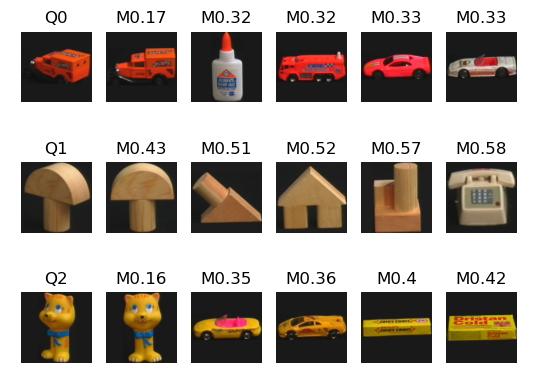
\includegraphics[width=.7\textwidth]{best_match}
\caption{Results of the matches using the best parameters}
\label{fig:best-match}
\end{figure}

From the results we can observe that with the greyvalue histogram type the performance are pretty bad since it's the one that uses the least amount of informations.
With the DxDy histogram type we get acceptable performance only when used with the intersect distance.

Finally, the RG and RGB histogram types have a similar trend: they perform well with the  intersect measure and only in particolar cases with the other distance types, but the more complexity of the RGB histogram type produces better results.

\section*{Question 4.b}

From the plots we can see that the greyvalue and dxdy histogram types are the worst, since the ideal curve will have a high recall and precision.
Instead, the rg and rgb curves seems to have the same trend so we plotted an in detail comparison in the Figure \ref{fig:rpc_rg_vs_rgb} where we can confirm that the two histogram types are similar.

\begin{figure}[ht]
\centering
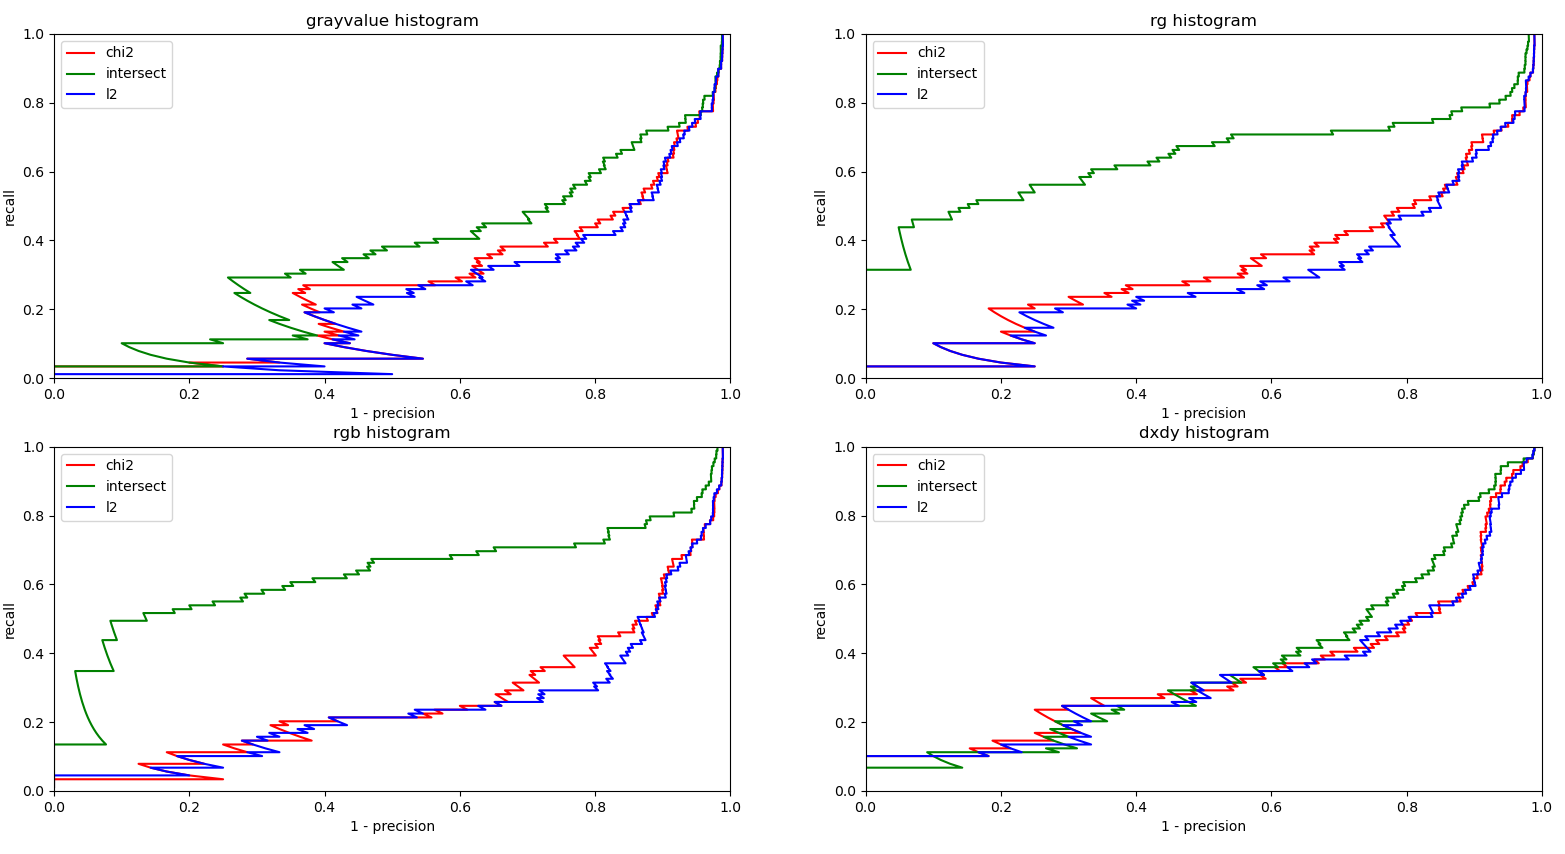
\includegraphics[width=\textwidth]{rpc_all}
\caption{RP curve for each histogram type and 30 as number of bins}
\label{fig:rpc_all}
\end{figure}

\begin{figure}[ht]
\centering
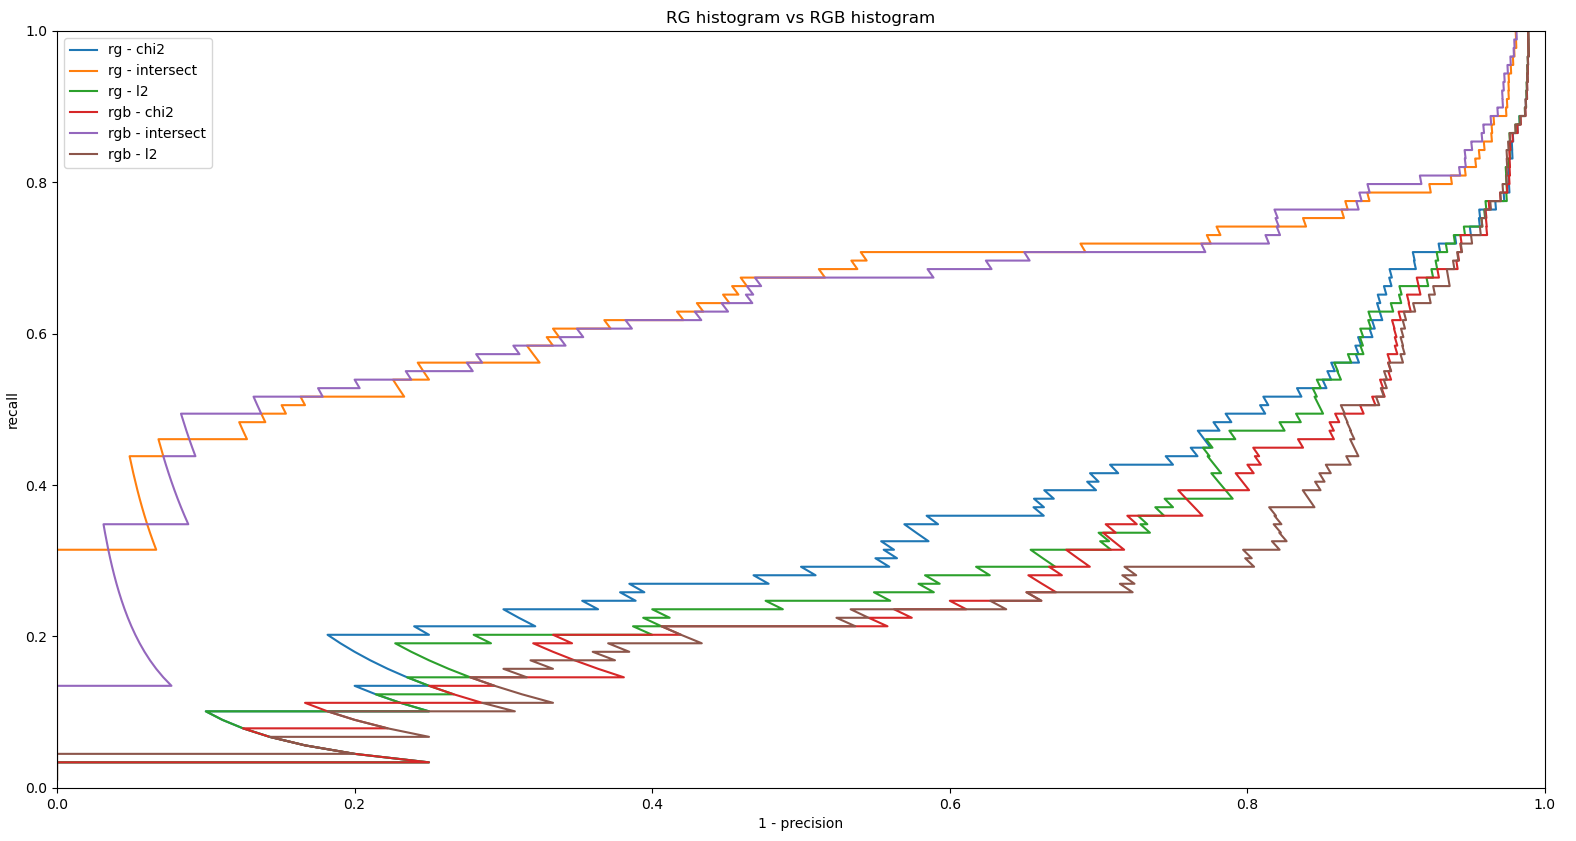
\includegraphics[width=\textwidth]{rpc_rg_vs_rgb}
\caption{Comparison of the RP curve of the rg and rgb histogram type in the Figure \ref{fig:rpc_all}}
\label{fig:rpc_rg_vs_rgb}
\end{figure}

\end{document}